\chapter{VISÃO COMPUTACIONAL}

É apresentado neste Capítulo uma introdução da área de Visão Computacional, mostrando seu conceito e como o assunto tem se desenvolvido ao longo dos anos. Ainda, são apresentadas áreas de aplicação prática do assunto. Por fim, é apresentada a estrutura desse domínio, separada hierarquicamente por subáreas de estudo.

\section{Conceito}

A área de Visão Computacional tem como principal função recriar o sistema de visão de um ser humano, de modo que seja possível descrever o cenário percebido por esse sistema. \citeonline{TRUCCO} destacam que encontrar uma definição incontroversa a respeito de Visão Computacional é uma tarefa difícil, por ser uma disciplina com diferentes perspectivas. Definir um conceito claro sobre o assunto se torna mais fácil ao buscar quais os problemas a Visão Computacional propõe resolver e como isso é feito. Sob a perspectiva de \citeonline{SHAPIRO}, a Visão Computacional tem como objetivo tomar decisões úteis a respeito de objetos físicos reais e cenas com base em imagens sensoriais.

\citeonline{TRIVEDI} contextualizam a área de Visão Computacional junto a dois outros campos de estudo: neurofisiologia e psicologia perceptual. A neurofisiologia tenta entender como mecanismos neurais dos sistemas biológicos e sensoriais funcionam. A psicologia perceptual tenta entender os casos psicológicos direcionando a tarefa de percepção. Já a Visão Computacional investiga os casos computacionais e algorítmicos associados a aquisição, processamento e compreensão da imagem.

Nesse contexto é entendido que o campo de estudo de Visão Computacional trata-se de uma ciência que busca tornar possível a compreensão e interpretação de imagens, e assim adquirir informações relevantes a seu respeito, utilizando métodos científicos, comprovando e documentando resultados encontrados. É importante destacar que a área está intimamente relacionada a outros campos de estudo como inteligência artificial, matemática, neurobiologia e física.

\section{Histórico}

As primeiras ideias relacionadas a Visão Computacional são de 1950 em trabalhos de Levialdi, que buscava analisar imagens provenientes de experimentos físicos em câmaras de bolhas através de técnicas de Processamento de Imagem \cite{JOLION}.

Ainda segundo \citeonline{JOLION}, muitos pesquisadores da área acreditavam que o problema da Visão Computacional seria resolvido rapidamente. Um dos problemas fundamentais é que uma imagem bidimensional de uma cena não possibilita que se construa uma representação tridimensional da cena em questão, pois não existem equações geométricas suficientes para encontrar todas as incógnitas necessárias à reconstrução.

Apesar de muitos estudos importantes terem sido realizados, poucos frutos foram colhidos. Os principais pesquisadores descobriram que, para simular a percepção na máquina, seriam necessárias mais informações de como o cérebro interpreta as imagens e ferramentas para melhor desempenho no processamento \cite{REINALDO}.

A partir dos anos 60, o incentivo para pesquisas em novas tecnologias computacionais causado pelas disputas políticas da Guerra Fria, permitiu um avanço em Visão Computacional com maior foco nas áreas de restauração, seletividade e transmissão de imagens. Na década de 70, surgiram os moldes de como esta área é apresentada hoje. Nessa época aumentaram as pesquisas sobre Processamento de Imagem, focadas em ordenação, melhorias na qualidade ou restauração e análise de imagem \cite{ANDREWS}. Tempos depois, \citeonline{MARR} propôs uma investigação computacional para a representação humana e processamento da informação visual, sendo a primeira metodologia completa para a Visão Computacional \cite{JOLION}. A partir dessas ideias, novos paradigmas surgiram, buscando melhorar a forma como o problema da Visão Computacional era descrito \cite{BLACK} \cite{BAJCSY} \cite{BALLARD} \cite{ALOIMONOS}.

\section{Cenário atual}
\label{section:cenario_atual}

Ainda hoje, a Visão Computacional é considerada uma ciência em desenvolvimento, pois não foi encontrado um modelo genérico de percepção visual para ser utilizado na prática. A solução encontrada ainda vem sendo a utilização de conjuntos de algoritmos específicos para determinados tipos de tarefas na interpretação de uma imagem. \citeonline{SZELISKI} afirma que para projetar algoritmos de Visão Computacional é necessário uma análise do problema proposto e das limitações na representação da imagem formada.

Com o crescimento significativo de estudos na área de Visão Computacional, encontrar soluções que auxiliam o trabalho em outras áreas vem se tornando cada vez mais comum. Hoje já é possível encontrar aplicações que utilizam sistemas de Visão Computacional para realizar diversas tarefas, a fim de auxiliar ou substituir as que antes eram executadas por pessoas. Dentre essas aplicações encontram-se:

\begin{itemize}
    \item{Reconhecimento óptico de caracteres;}
    \item{Inspeção ou controle de qualidade de produtos;}
    \item{Construção de modelos 3D;}
    \item{Medicina (medicina remota, reconstrução 3D, identificação de padrões orgânicos);}
    \item{Direção autônoma;}
    \item{Captura de movimentos;}
    \item{Vigilância;}
    \item{Reconhecimento de biometria;}
    \item{Análise de imagens geográficas.}
\end{itemize}

\section{Estrutura da área de Visão Computacional}

O diagrama da Figura \ref{img:diagrama_vc} separa os processos da Visão Computacional hierarquicamente e divididos em três campos. De modo geral, cada um dos componentes apresentados tem uma finalidade dentro da Visão Computacional. As aplicações apresentadas na Seção \ref{section:cenario_atual} são resultados da união de vários desses componentes, somando ao uso de algoritmos que buscam o melhor resultado para cada área em questão.

\begin{figure}[H]
    \centering
    {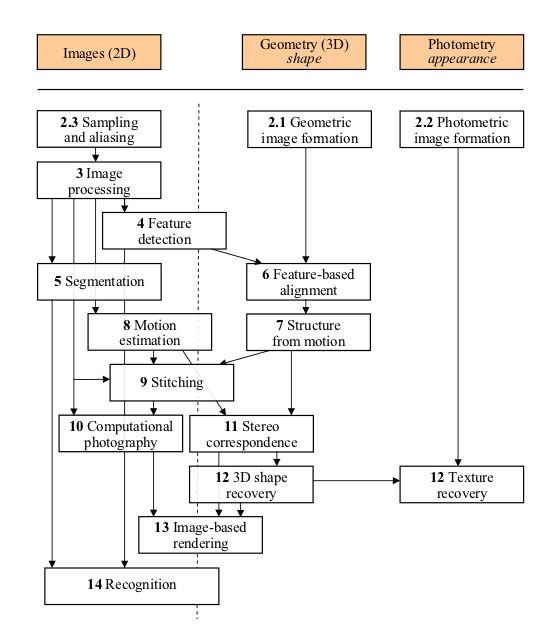
\includegraphics[scale=0.75]{figuras/diagrama_vc}}
    \caption{Divisão das áreas da Visão Computacional, relacionadas de acordo com suas dependências. Adaptado de \cite{SZELISKI}.}
    \label{img:diagrama_vc}
\end{figure}

Observando da esquerda para direita, podem ser vistos os três campos da Visão Computacional, divididos como: Imagens (\textit{Images}), Geometria (\textit{Geometry}) e Fotometria (\textit{Photometry}). A primeira área (\textit{Images}) cuida de problemas em um universo bidimensional. O tópico sobre Amostragem e Serrilhamento (\textit{Sampling and aliasing}) trata de questões referentes a fotografia digital. A parte de Processamento de Imagem (\textit{Image Processing}) foca na melhoria da qualidade da imagem para manipulações em sistemas de Visão Computacional. Já o processo de Detecção por Características (\textit{Feature Detection}), como o próprio nome sugere, dispõe de técnicas para reconhecimento de características em imagens.

Ainda, existe o processo de Segmentação (\textit{Segmentation}), que aborda técnicas de segmentação de imagens. Em outras palavras, esse processo é responsável por separar regiões relevantes de uma imagem. A Estimativa de Movimento (\textit{Motion Estimation}) é utilizada para alinhamento geométrico e calibração de câmeras e que em alguns momentos também pode ser encontrado em tarefas de um universo 3D (tridimensional). O processo de Junção de Imagens (\textit{Stitching}) cuida da criação de novas imagens a partir de uma ou mais imagens de entrada. Esse procedimento é bastante usado na área de mapas digitais e fotos de satélite, e tal como o processo de Estimativa de movimento, pode também ser utilizado em ambientes 3D.

Diretamente ligado ao processo de Junção de Imagens, encontra-se a Fotografia Computacional (\textit{Computational Photography}), que refere-se a captura, processamento e técnicas de manipulação da imagem computacional que melhoram ou aumentam a capacidade da fotografia digital. Como último processo de imagens 2D (bidimensional), temos o processo de Reconhecimento (\textit{Recognition}), tendo com tarefa principal analisar uma cena e reconhecer objetos.

Na próxima coluna, encontra-se os processos que tratam, em sua maioria, de casos em universo 3D. A Formação da Imagem Geométrica (\textit{Geometric image formation}) trata pontos, linhas e planos e como esses podem ser mapeados em imagens. A parte de Alinhamento Baseado em Características (\textit{Feature-based alignment}) trata das características recuperadas de imagens em processos anteriormente utilizados e busca identificá-las em outras diferentes imagens. Feito o processo de Alinhamento Baseado em Características, pode-se então utilizar o conjunto de técnicas no processo de Estrutura a Partir do Movimento (\textit{Structure from motion}), que cuida de encontrar estruturas tridimensionais de um objeto através de sinais de movimento continuamente.

Prosseguindo, está o processo Correspondência Estéreo (\textit{Stereo correspondence}), que pode ser entendido como a parte da Visão Computacional que analisa objetos em uma cena, sendo tratados por diversos pontos de vista. Na mesma linha de reconstrução de modelos 3D, está o componente de recuperação de formas 3D (\textit{3D shape recovery}). Diferente da Correspondência estéreo, esse componente funde diversas imagens de profundidade e de alcance. Por fim, está o componente da Renderização Baseada em Imagem (\textit{Image-based rendering}), diretamente ligado aos dois universos. O conjunto de técnicas nesse tópico cuida da geração de modelos 3D a partir de imagens 2D.

Além dessas áreas núcleo dos sistemas de Visão Computacional, existe a Fotometria, classe de técnicas de medição, que realiza a medição de objetos do mundo real usando apenas imagens. Em seus processos, estão a Formação da Imagem Fotométrica (\textit{Photometric image formation}) e a Recuperação de Texturas (\textit{Texture recovery}). O primeiro, descreve como os sensores geram valores de cor e intensidade, e como esses são formados em uma imagem. O segundo, está ligado a aparência dos objetos da superfície, após terem sido gerados como modelo 3D.

No Capítulo seguinte, são detalhados os principais processos de Visão Computacional. Por se tratar de disciplinas essenciais para o entendimento da área de Visão Computacional, foram escolhidos processos referentes ao universo bidimensional. A abordagem desses tópicos tem como finalidade servir de base conceitual para o desenvolvimento do estudo de caso, exposto no Capítulo 5.
